\section{E-Logbook}
E-Logbook adalah sebuah buku elektronik untuk mencatat catatan/dokumen penting secara detail setiap aktivitas yang berisi masalah-masalah yang membutuhkan tindak lanjut dari pihak yang terlibat dalam satu hari penuh. Seluruh pegawai sebaiknya membaca buku ini agar mengetahui kegiatan, kerusakan, dan target pekerjaan apa saja yang dilakukan hari sebelumnya. Ada beberapa manfaat e-logbook antara lain:
\begin{enumerate}
\item bahan bukti untuk merekap seluruh aktivitas
\item bahan pembuatan laporan kegiatan
\item alat untuk memudahkan pegawai dalam merekap kegiatan
 \end{enumerate}

Hal yang perlu di isi dalam e-logbook ini antara lain:
\begin{enumerate}
\item Hari, tanggal dan tahun
\item Nama pegawai yang dinas pada hari tersebut
\item Nama vendor yang dinas pada hari tersebut
\item Penerbangan hari ini
\item Kegiatan
\item Kerusakan
\item Target pekerjaan
\end{enumerate}


\subsection{Mengaktifkan MySQLi}
Kenapa disini kita membahas tentang cara mengaktifkan MySQLi karena PHP 5 keatas default-nya menggunakan platform MySQLi untuk menggunakan berbagai fungsi pada database MySQL. MySQLi adalah sebuah class di PHP, jadi pastikan bahwa versi PHP kita sudah 5 keatas yaa.
Keunggulan menggunakan MySQLi ketimbang dengan MySQL:
\begin{enumerate}
\item Dukungan baru untuk keperluan transaksi
\item Prosedur interface
\item Susunan laporan lebih tersusun
\item Debugging lebih ditingkatkan
\item Dapat memproses dalam waktu yang lebih singkat
\end{enumerate}

Nah itu beberapa keunggulan menggunakan MySQLi. Dan sekarang kita akan membahas cara mengaktifkan MySQLi pada PHP.
Untuk mengaktifkan MySQLi, langkah pertama update dahulu versi PHP kita ke PHP 5 keatas. kemudian cari file php.ini biasanya terdapat di folder C lalu folder xampp lalu folder php kemudian buka file php.ini menggunakan editor seperti notepad++, sublime text, dan adobe dreamweaver. Tambahkan skrip extension=php\_mysqli.dll pada file php.ini. Namun pada file php.ini sudah ada skrip extension=php\_mysqli.dll dan terdapat tanda ; (tanpa tanda kutip) di depanya, maka kita cukup menghapus tanda ; tersebut lalu simpan file php.ini yang sudah di edit. Jangan lupa untuk restart server apachenya.

\subsection{Cara Install XAMPP}
Agar dapat menjalankan sistem yang akan dibuat, kita harus menginstall aplikasi web server yang mendukung PHP ini serta aplikasi untuk database MySQL. Untungnya terdapat banyak aplikasi yang menghandle program ini, salah satunya yaitu XAMPP. Aplikasi XAMPP adalah aplikasi yang dapat menghandle banyak aplikasi lain yang dibutuhkan untuk pengembangan web. Nama XAMPP adalah singkatan dari X (huruf X berarti cross-platform), A (Apache web server), M (MySQL), P (PHP), dan P (Perl). Selain beberapa aplikasi tersebut XAMPP menyediakan modul lain seperti OpenSSL dan phpMyAdmin.
\par
Cara mendownload XAMPP terbaru bisa di situs resminya yaitu www.apachefriends.org. Untuk versi terbaru sudah support untuk PHP 7, silahkan pilih download sesuai dengan sistem operasi yang kita pakai.

\begin{figure}[h]
\centering

\includegraphics[scale=0.5]{figures/xampp}
\caption{Versi Terbaru XAMPP}
\end{figure}

File xampp-windows-x64-7.3.4-0-VC15-installer berukuran cukup besar, sekitar 149MB. Simpanlah file ini dimana kita inginkan.
Setelah file XAMPP sudah di download, kita akan menginstallnya dengan cara double klik pada aplikasi tersebut dan akan mucul peringatan sebagai berikut.

 \begin{figure}[h]
\centering
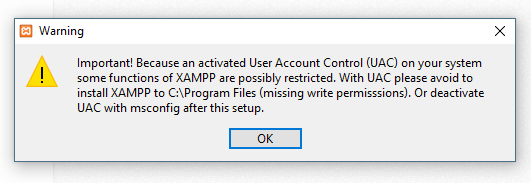
\includegraphics[scale=0.5]{figures/uac}
\caption{User Account Control}
\end{figure}

Peringatan ini berkaitan dengan keamanan pada versi Windows Vista keatas dan jika XAMPP akan di install pada folder C mungkin akan terjadi pembatasan hak akses terhadap XAMPP yang berjalan tidak normal. Silahkan klik tombol OK untuk melanjutkan install maka akan muncul jendela awal install. Silahkan klik next.

 \begin{figure}[h]
\centering
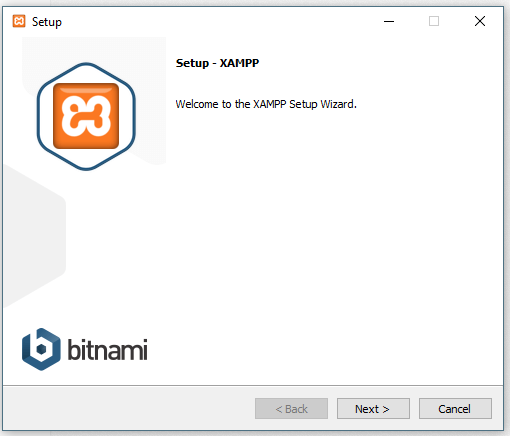
\includegraphics[scale=0.5]{figures/jendelaawal}
\caption{Jendela Awal}
\end{figure}

Jendela selanjutnya adalah Select Component. Dalam jendela ini kita dapat memilih modul atau aplikasi apa saja yang akan kita install. Dalam tahap ini kita akan menceklis semua pilihan selanjutnya klik next untuk melanjutkan.

\begin{figure}[h]
\centering
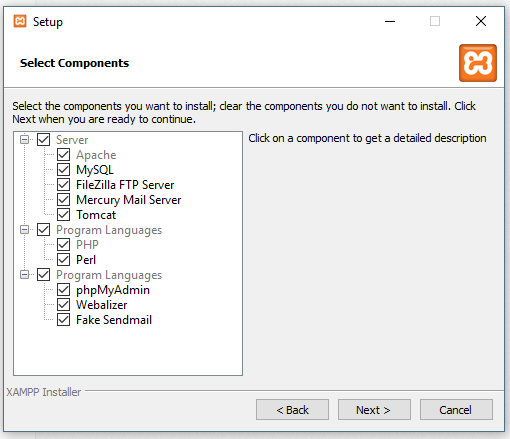
\includegraphics[scale=0.5]{figures/selectcomponent}
\caption{Select Component}
\end{figure}

Jendela selanjutnya adalah Installation Folder. Dalam jendela ini kita dapat mengubah lokasi dimana kita akan menyimpan file-file XAMPP. Sebagai contoh kita akan menyimpan file XAMPP di drive E dengan nama folder xampp agar mudah di ingat. Untuk melanjutkan klik next.

\begin{figure}[h]
\centering
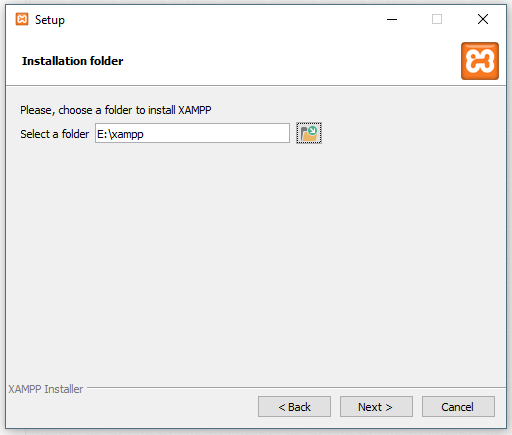
\includegraphics[scale=0.5]{figures/installationfolder}
\caption{Installation Folder}
\end{figure}

Jendela berikutnya adalah Bitnami for XAMPP. Dalam hal ini XAMPP menawarkan Bitnami sebagai cara cepat untuk install CMS seperti wordpress, drupal, dan joomla. Kemudian klik next.

\begin{figure}[h]
\centering
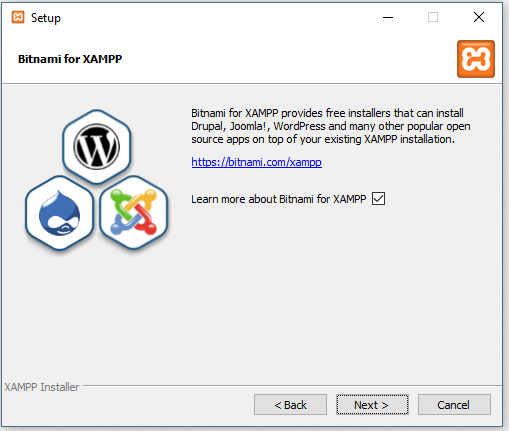
\includegraphics[scale=0.5]{figures/bitnamiforxampp}
\caption{Bitnami for XAMPP}
\end{figure}

Jendela berikutnya adalah pemberitahuan bahwa kita siap untuk menginstall XAMPP, Klik next dan XAMPP akan memulai  proses penginstallan.

\begin{figure}[h]
\centering
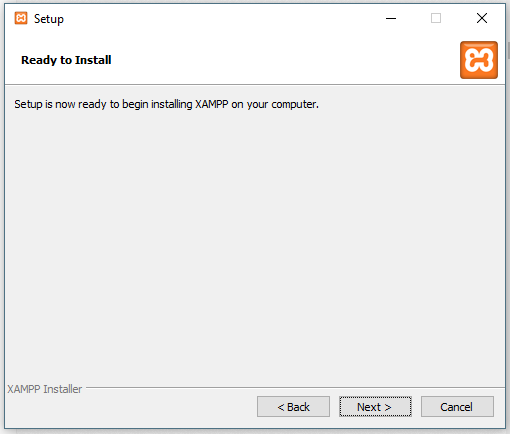
\includegraphics[scale=0.5]{figures/readytoinstall}
\caption{Ready to Install}
\end{figure}

\begin{figure}[h]
\centering
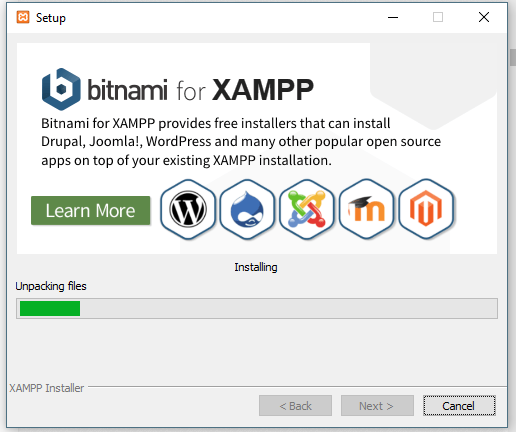
\includegraphics[scale=0.5]{figures/setup}
\caption{Proses Penginstallan}
\end{figure}

Setelah proses penginstallan hampir selesai akan muncul jendela Windows Security Alert pada gambar 5.9 karena Windows Defender Firewall mendenteksi Apache HTTP Server. Untuk lanjut klik Allow access.

\begin{figure}[h]
\centering
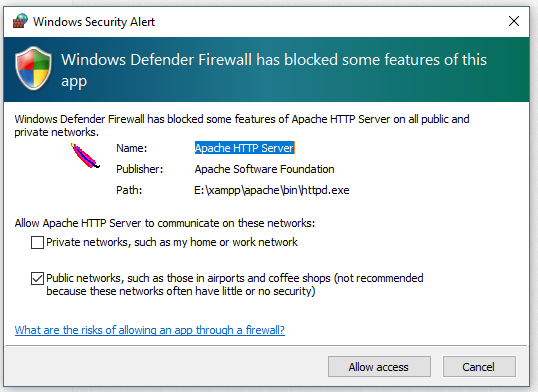
\includegraphics[scale=0.5]{figures/windowssecurityalert}
\caption{Windows Security Alert}
\end{figure}

Proses penginstallan XAMPP sudah selesai pada gambar 5.10 maka akan muncul jendela Completing, dalam bagian ini kita dapat memilih untuk langsung menggunakan XAMPP atau tidak. Jika ingin langsung memakai, ceklis pada Do you want to start the Control Panel now? lalu klik finish. Jika tidak maka hilangkan ceklis dari  Do you want to start the Control Panel now? lalu klik finish.

\begin{figure}[h]
\centering
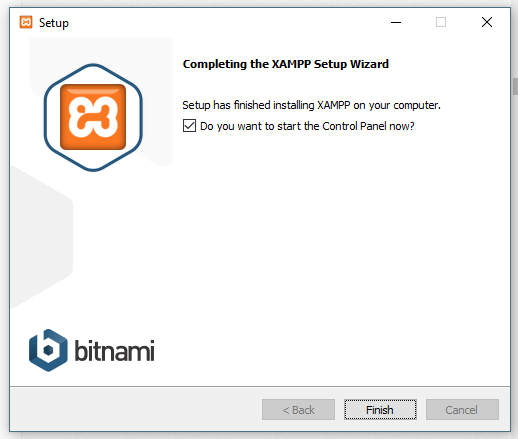
\includegraphics[scale=0.5]{figures/selesaiinstall}
\caption{Selesai Install}
\end{figure}

\subsection{Menguji Instalasi XAMPP}
Sesuai dengan namanya, jendela XAMPP Control Panel adalah jendela yang digunakan untuk mengontrol apa saja modul atau aplikasi apa saja yang ingin kita jalankan. Jika ingin membuka manual maka kita dapat membuka dengan cara dari menu Start->All Programs->XAMPP->XAMPP Control Panel. Untuk menguji instalan XAMPP ini, silahkan klik tombol Start pada modul apache dan MySQL. Jika tidak ada masalah maka akan tampil warna hijau pada bagian modul ini.

\begin{figure}[h]
\centering
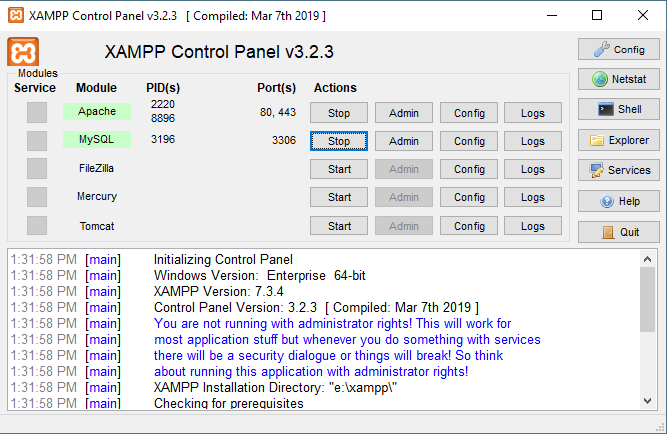
\includegraphics[scale=0.5]{figures/controlpanel}
\caption{XAMPP Control Panel}
\end{figure}

Selanjutnya buka web browser dan ketikan localhost pada address bar kemudian enter maka akan muncul dengan otomatis localhost/dashboard semuanya telah terinstall dengan baik.

\begin{figure}[h]
\centering
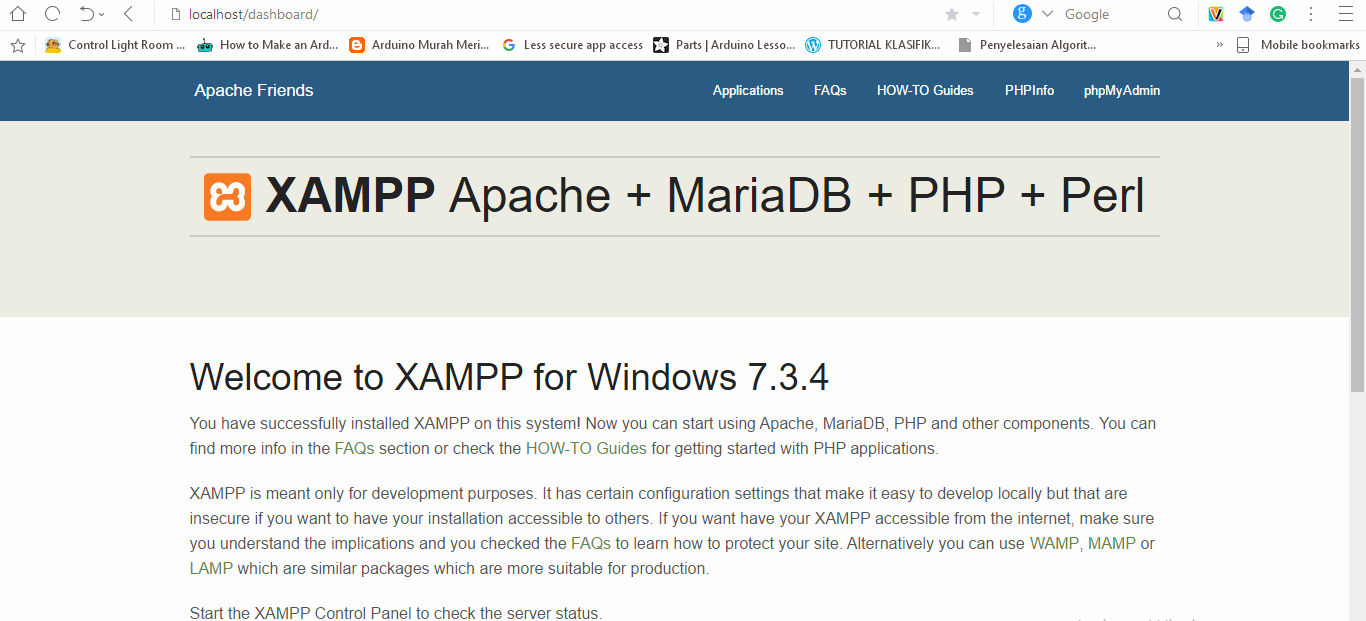
\includegraphics[scale=0.3]{figures/dashboard}
\caption{Localhost Dashboard}
\end{figure}

Jika ingin melihat versi PHP kita secara mendalam silahkan klik PHPInfo di pojok kanan atas. Disini kita dapat melihat bahwa PHP yang kita pakai sudah versi 7.3.4.

\begin{figure}[h]
\centering
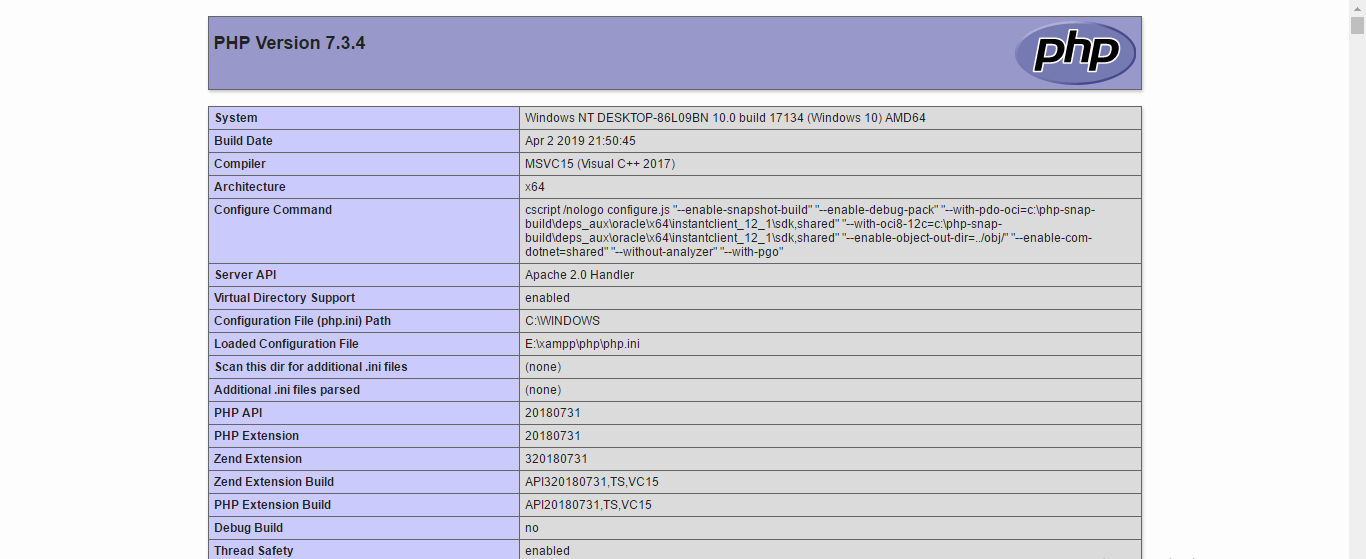
\includegraphics[scale=0.4]{figures/versiphp}
\caption{Versi PHP}
\end{figure}

\subsection{Membuat Database}
Secara umum, tipe website bisa dibedakan menjadi dua yaitu web statis dan web dinamis. Web statis adalah web yang tetap dalam arti tampilan, navigasi, dan konten tidak dapat berubah dengan otomatis. Ketika kita ingin mengupdate sebuah kegiatan akan tetapi kita harus membuka file yang aslinya. Umumnya kegiatan yang ditampillkan tetap untuk jangka waktu satu hari - satu hari. Tipe website ini biasanya hanya berupa tag html saja, jadi diperlukan database yang digunakan untuk menyimpan data.
\par
Selain memanfaatkan tag html, website yang menggunakan flash juga bisa dikategorikan sebagai web statis, meskipun ada sebagian kecil yang sudah memiliki database dalam mengelola konten tidak perlu membuka sebuah file tertentu namum hanya menambahkan pada form yang telah disiapkan dan tersimpan di database. Sama halnya dengan e-logbook ini harus ada database yang dibuat.
\begin{enumerate}
\item Untuk membuat database kita pertama kali harus membuka aplikasi XAMPP yang sudah terinstall dan klik start pada Apache serta MySQL.

 \begin{figure}[h]
\centering
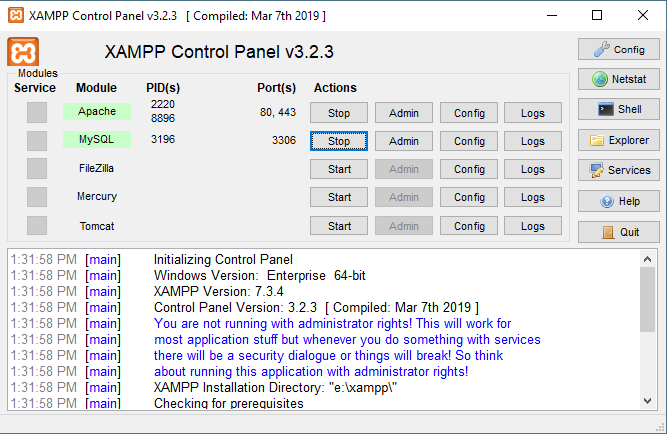
\includegraphics[scale=0.5]{figures/controlpanel}
\caption{XAMPP Control Panel}
\end{figure}

\item Jika sudah berjalan maka selanjutnya buka web browser kesayangan kita lalu ketikan https://localhost/phpmyadmin

 \begin{figure}[h]
\centering
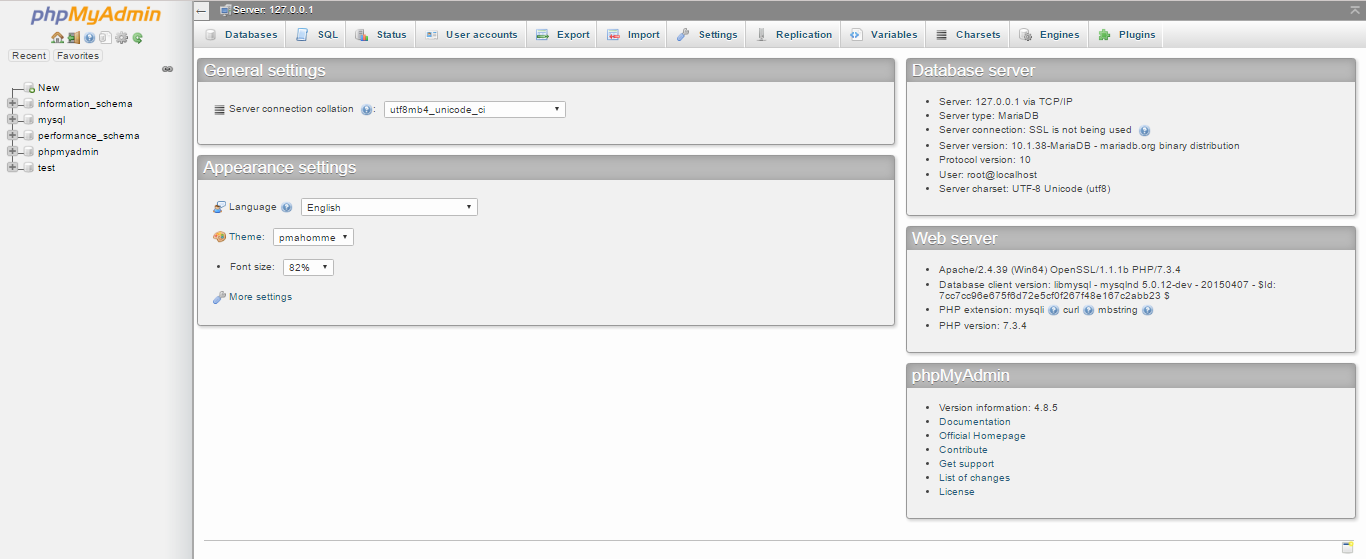
\includegraphics[scale=0.35]{figures/phpmyadmin}
\caption{Halaman Utama}
\end{figure}

\item Setelah itu, klik databases lalu ketikkan elban lalu klik create

 \begin{figure}[h]
\centering
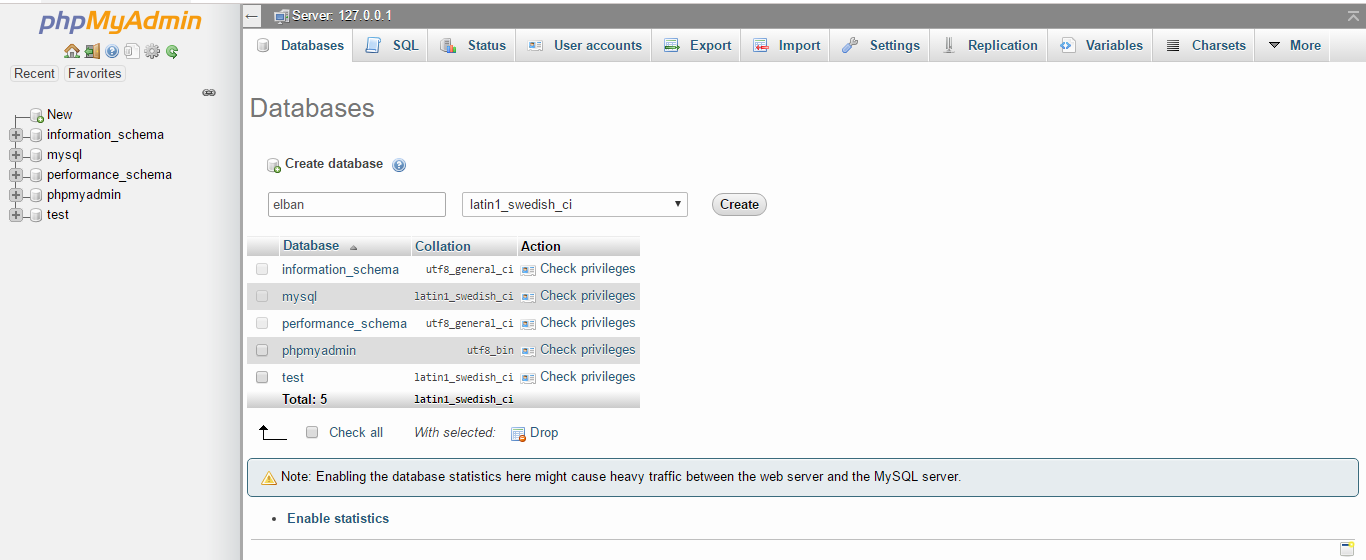
\includegraphics[scale=0.35]{figures/databases}
\caption{Create Database}
\end{figure}

\item Setelah database dibuat lalu belum ada table, klik SQL lalu masukan codingan berikut

\begin{lstlisting}
CREATE TABLE IF NOT EXISTS `logbook` (
  `id_logbook` int(10) NOT NULL,
  `tanggal` date NOT NULL,
  `petugas` varchar(100) NOT NULL,
  `vendor` varchar(100) NOT NULL,
  `penerbangan` varchar(100) NOT NULL,
  `kegiatan` varchar(500) NOT NULL,
  `point_kerusakan` varchar(200) NOT NULL,
  `target_pekerjaan` varchar(200) NOT NULL,
  `id_user` tinyint(1) NOT NULL
) ENGINE=InnoDB AUTO_INCREMENT=4 DEFAULT CHARSET=latin1;

--
-- Dumping data for table `logbook`
--

INSERT INTO `logbook` (`id_logbook`, `tanggal`, `petugas`, `vendor`, `penerbangan`, `kegiatan`, `point_kerusakan`, `target_pekerjaan`, `id_user`) VALUES
(2, '2019-03-31', 'M. Arif S, Vania & Rismayadi', 'Anto (CUPPS) Hisyam', 'Citylink KJT - KNO', 'PM di SCP 2 Inter Line 1', 'Master Clok Gate 4, XRAY BHS Internasional', 'Master Clock Gate 4', 12),
(3, '2019-03-28', 'M. Arif S & Vania', 'Anto (CUPPS) Hisyam', 'KJT - KNO (Cancelled)', 'PM', 'Master clock gate 4 off', 'Master CloCk gate 4', 12);

-- --------------------------------------------------------

--
-- Table structure for table `pegawai`
--

CREATE TABLE IF NOT EXISTS `pegawai` (
  `id_pegawai` int(10) NOT NULL,
  `pegawai` varchar(100) NOT NULL
) ENGINE=InnoDB AUTO_INCREMENT=16 DEFAULT CHARSET=latin1;

--
-- Dumping data for table `pegawai`
--

INSERT INTO `pegawai` (`id_pegawai`, `pegawai`) VALUES
(1, 'M. Arif S'),
(2, 'M. Arif S & Vania'),
(3, 'M. Arif S, Vania & Hafiz'),
(4, 'M. Arif S, Vania & Rismayadi'),
(5, 'M. Arif S & Hafiz'),
(6, 'M. Arif S & Rismayadi'),
(7, 'M. Arif S, Vania, Hafiz & Rismayadi'),
(8, 'Vania'),
(9, 'Vania & Hafiz'),
(10, 'Vania & Rismayadi'),
(11, 'Vania, Hafiz & Rismayadi'),
(12, 'Hafiz'),
(13, 'Hafiz & Rismayadi'),
(14, 'Rismayadi'),
(15, 'M. Arif S, Hafiz & Rismayadi');

-- --------------------------------------------------------

--
-- Table structure for table `user`
--

CREATE TABLE IF NOT EXISTS `user` (
  `id_user` tinyint(2) NOT NULL,
  `username` varchar(30) NOT NULL,
  `password` varchar(35) NOT NULL,
  `nama` varchar(50) NOT NULL,
  `alamat` varchar(150) NOT NULL,
  `hp` varchar(20) NOT NULL,
  `level` tinyint(1) NOT NULL
) ENGINE=InnoDB AUTO_INCREMENT=14 DEFAULT CHARSET=latin1;

--
-- Dumping data for table `user`
--

INSERT INTO `user` (`id_user`, `username`, `password`, `nama`, `alamat`, `hp`, `level`) VALUES
(1, 'admin', '21232f297a57a5a743894a0e4a801fc3', 'Luqman Nurfajri', 'Ciwarugotham', '089634530333', 1),
(13, 'vania', '081c2ce8528c443cc4be69d4096c9778', 'Vania R', 'Kertajati', '-', 1);

--
-- Indexes for dumped tables
--

--
-- Indexes for table `logbook`
--
ALTER TABLE `logbook`
  ADD PRIMARY KEY (`id_logbook`);

--
-- Indexes for table `pegawai`
--
ALTER TABLE `pegawai`
  ADD PRIMARY KEY (`id_pegawai`);

--
-- Indexes for table `user`
--
ALTER TABLE `user`
  ADD PRIMARY KEY (`id_user`);

--
-- AUTO_INCREMENT for dumped tables
--

--
-- AUTO_INCREMENT for table `logbook`
--
ALTER TABLE `logbook`
  MODIFY `id_logbook` int(10) NOT NULL AUTO_INCREMENT,AUTO_INCREMENT=4;
--
-- AUTO_INCREMENT for table `pegawai`
--
ALTER TABLE `pegawai`
  MODIFY `id_pegawai` int(10) NOT NULL AUTO_INCREMENT,AUTO_INCREMENT=16;
--
-- AUTO_INCREMENT for table `user`
--
ALTER TABLE `user`
  MODIFY `id_user` tinyint(2) NOT NULL AUTO_INCREMENT,AUTO_INCREMENT=14;
\end{lstlisting}

\end{enumerate}

\section{Struktur Dasar PHP}
Pada awalnya PHP adalh kependekan dari Personal Home Page (Situs personal). PHP pertama kali dibuat oleh Rasmus Lerdorf pada tahun 1995. Pada saat itu PHP masih bernama Form Interpreted (FI), yang wujudnya berupa sekumpulan skrip yang digunakan untuk mengolah data formulir dari web. Selanjutnya Rasmus merilis kode sumber tersebut untuk umum dan menamakannya PHP/FI. Dengan perilisan kode sumber ini menjadi sumber yang terbuka, maka banyak pemrogram yang ikut tertarik untuk ikut mengembangkan PHP.
\par
Pada November 1997, dirilis lah PHP/FI 2.0. Pada rilisan ini, interpreter PHP sudah diimplementasikan dalam program C. Dalam rilis ini disertakan juga modul-modul ekstensi yang meningkatkan kemampuan PHP/FI secara signifikan. Pada tahun 1997, ada sebuah perusahaan bernama Zend menulis ulang interpreter PHP menjadi lebih bersih, lebih baik, dan lebih cepat. Kemudian pada Juni 1998, perusahaan tersebut dapat merilis interpreter baru untuk PHP dan meresmikan rilis tersebut sebagai PHP 3.0 dan singkatan PHP diubah menjadi akronim berulang PHP: Hypertext Preprocessing. Pada pertengahan tahun 1999, Zend merilis interpreter PHP baru dan rilis tersebut dikenal dengan PHP 4.0. PHP 4.0 adalah versi PHP yang paling banyak dipakai pada awal abad ke-21. Versi ini banyak dipakai disebabkan kemampuannya untuk membangun aplikasi web kompleks tetapi tetap memiliki kecepatan dan stabilitas yang tinggi. 
\par
Pada Juni 2004, Zend merilis PHP 5.0. Dalam versi ini, inti dari interpreter PHP mengalami perubahan besar. Versi ini juga memasukkan model pemrograman berorientasi objek ke dalam PHP untuk menjawab perkembangan bahasa pemrograman ke arah paradigma berorientasi objek. Server web bawaan ditambahkan pada versi 5.4 untuk mempermudah pengembang menjalankan kode PHP tanpa menginstall software server. Versi terbaru dan stabil dari bahasa pemograman PHP saat ini adalah versi 7.0.16 dan 7.1.2 yang resmi dirilis pada tanggal 17 Februari 2017.

\subsection{Variabel}
Variabel ini digunakan untuk menyimpan sebuah nilai, data atau informasi.
\begin{enumerate}
\item Nama dari variabel diawali dengan tanda dollar \$.
\item Panjang dari variabel tidak terbatas.
\item Setelah tanda \$ .
\item Tidak perlu untuk dideklarasikan atau compile.
\item Tidak boleh mengandung spasi.
\end{enumerate}
Contoh:
\begin{lstlisting}
<?php
$npm="1154054";
$nama=' Luqman Nurfajri';
echo"npm : ".npm ."<br>;
echo"nama: &nama";
?>
\end{lstlisting}

\subsection{Tipe Data}
Pada PHP, tipe data dari variabel tergantung kondisi yang dialami oleh programmer itu sendiri. Akan tetapi secara otomatis dapat ditentukan oleh PHP. PHP telah mendukung 8 buah tipe data primitif yaitu:
\begin{enumerate}
\item Boolean.
\item Integer.
\item Float.
\item String.
\item Array.
\item Object.
\item Resource.
\item NULL.
\end{enumerate}
Contoh:
\begin{lstlisting}
<?php
$npm = "1154054";
$nama = ' Luqman Nurfajri';
$umur= 22;
$nilai = 98.75;
$status = TRUE;
echo"NPM : ". $npm ."<br>;
echo"Nama:  $nama";
print "Umur : " . $umur; print "<br>";
printf ("Nilai: %.3f<br>"), $nilai);
if ($status)
echo "Status: Aktif";
else
echo "Status: Tidak Aktif:;
?>
\end{lstlisting}

\subsection{Konstanta}
Konstanta adalah sebuah variabel konstan yang nilainya tidak berubah-ubah. Untuk mendefinisikan konstanta dalam PHP, menggunakan fungsi define() .
Contoh:
\begin{lstlisting}
<?php
define ("Nama", "Luqman Nurfajri";
define ("Nilai", 98.75);
echo"Nama : ".Nama .<br>;
echo"Nilai: " .Nilai";
?>
\end{lstlisting}


\subsection{Struktur Kondisi Dan Perulangan}
\subsubsection{Struktur Kondisi IF}
Kondisi IF adalah kondisi dimana sebuah data yang apabila kondisinya jika dan hanya nilai kebenaran dari hasil yang dibuat adalah benar, tetapi jika kondisi yah diuji salah maka sistem / program akan tidak menanggapi. Contoh:
\begin{lstlisting}
 if (bebas) {
                pernyataan benar
}
\end{lstlisting}
Dari skrip diatas parameter IF ini dapat kita gunakan dalam PHP, buatlah file dengan nama \textbf{bebas.php}.
\begin{lstlisting}
<html>
<head>
<title> Test Kondisi IF </title>
   <body>
    <?php
         $bebas ="aih";

         if ($bebas == "aih") {
                echo "Buku ini semoga bermanfaat";
          }
         ?>
    </body>
</html>
\end{lstlisting}
 

\subsubsection{Struktur Kondisi IF ELSE}
Kondisi IF ELSE  digunakan untuk jika kondisi kita memiliki dua pilihan dari hasil yang berbeda, contohnya hasil yang keluar bernilai benar (\textit{true}) dan bernilai salah (\textit{false}). Secara standar sintaks seperti ini:
\begin{lstlisting}
if (bebas) {
    statement benar
} else {
     statement salah
}
\end{lstlisting}
Dari sintaks diatas kita dapat menyimpulkan bahwa, apabila \textbf{bebas} mendapatkan nilai yang sesuai maka \textit{statement} akan benar maka program yang akan dieksekusi benar dan jika \textbf{bebas} mendapatkan nilai salah maka yang dieksekusi adalah \textit{statement} salah. Berikut contoh penggunaan kondisi IF dan ELSE. Buatlah file dengan nama\textbf{ ifelse.php}:
\begin{lstlisting}
<html>
<head>
<title>Test Kondisi IF dan ELSE </title>
</head>
    <body>
        <?php
            $makan = "eat";
                 if ($makan=="eat")
                      echo "Makan adalah bahasa indonesia dari eat";
                 else {
                      echo "Makan bukan bahasa indonesia dari EAt";
                  }
          ?>
    </body>
</html>
\end{lstlisting}

\subsubsection{Struktur Kondisi Switch Dan Case}
Struktur kondisi SWITCH DAN CASE digunakan saat penyelesaian dari persoalan dengan jumlah kondisi yang banyak. Struktur ini dapat memeriksa nilai suatu variabel dengan SWITCH dan memeriksa kondisi dengan CASE. Contoh:
\begin{lstlisting}
switch ($var) {
case '1' : statement-1; break;
case '2' : statement-2; break;
....
}
\end{lstlisting}
Berikut contoh penggunaan kondisi SWITCH dan CASE. Buatlah file dengan nama\textbf{ swicase.php}:
\begin{lstlisting}
<?php
$day =date ("D");
switch ($day) {
    case 'Sun' : $hari= "Minggu" ; break;
    case 'Mon' : $hari= "Senin" ; break;
    case 'Tue' : $hari= "Selasa" ; break;
    case 'Wed' : $hari= "Rabu" ; break;
    case 'Thu' : $hari= "Kamis" ; break;
    case 'Fri' : $hari= "Jum'at" ; break;
    case 'Sat' : $hari= "Sabtu" ; break;
    default: $hari = "Kiamat" ;
}
echo "Hari ini hari <b>$hari</b>";
?>
\end{lstlisting}

\subsubsection{Struktur Perulangan For}
Struktur perulangan digunakan dalam kondisi membatasi perulangan. sebagai contoh disini kita mengulang kalimat "Semoga buku ini bermanfaat" sebanyak 50 kali. Buatlah file dengan nama \textbf{for.php}
\begin{lstlisting}
<?php
for ($i= 1; $i <= 50; $i++)
{
   echo "Semoga buku ini bermanfaat";
   echo "<br />";
}
?>
\end{lstlisting}

\subsubsection{Struktur Perulangan While}
Struktur perulangan while digunakan pada saat banyaknya perulangan tidak dapat kita pastikan.
Disini kita mengulang angka  1 sampai 14 sebagai contoh:  Buatlah file dengan nama \textbf{while.php}
\begin{lstlisting}
<?php
$i=1;
while ($i <= 14)
{
  echo "$i";
  echo "<br />";
  $i=$i+1;
}
?>
\end{lstlisting}

\subsubsection{Struktur Perulangan Do While}
Struktur Do While sebenernya lanjutan dari perulangan While, perbedaan keduanya dilihat dari posisi pengecakan kondisi. Apabila perulangan While kondisi yang dicek di awal maka perulangan Do While di akhir perulangan. Disini kita mengulang angka  1 sampai 14 sebagai contoh:  Buatlah file dengan nama \textbf{dowhile.php}
\begin{lstlisting}
<?php
$i=1;
do
{
  echo "$i";
  echo "<br />";
  $i=$i+1;
} while ($i <= 10);
?>
\end{lstlisting}

\subsubsection{Struktur Perulangan Foreach}
Array adalah sebuah tipe data yang sering digunakan dalam membuat program menggunakan PHP. Kemampuan array dalam menyimpan banyak data dalam satu variabel akan sangat berguna untuk menyederhanakan dan menghemat penggunaan variabel. Perulangan Foreach adalah perulangan khusus untuk membaca nilai dari array. Buatlah file dengan nama \textbf{foreach.php}
\begin{lstlisting}
<?php
$manusia = array("Luqman","Fajri","Ahmad","Fahmi","Mister");

foreach ($manusia as $val)
{
   echo "$value";
   echo "<br />";
}
?>
\end{lstlisting}

\subsubsection{Struktur Break Dan Continue}
Struktur \textbf{BREAK} dan \textbf{CONTINUE} sering digunakan dalam berbagai pekerjaan. Kedua struktur tersebut digunakan untuk mengatur bagaimana jalan dari pengulangan. Struktur \textbf{Break} digunakan untuk menghentikan jalan dari pengulangan sedangkan \textbf{continue} digunakan untuk menlanjutkan ke lankah selanjutnya tanpa menjalankan sisa perintah di dalam skrip pengulangan. Buatlah file dengan nama \textbf{breconti.php}
\begin{lstlisting}
<?php
 
for ($i=1; $i <10 ; $i++) {
    if ($i == 5)
       continue;
    if ($i == 8)
       break;
    echo "$i ";
}
 
?>
\end{lstlisting}
Jadi dari skrip diatas dapat disimpulkan bahwa perintah  \textbf{continue} akan melanjutkan proses pengulangan dan perintah \textbf{break} akan menghentikan proses. Dalam proses keduanya maka tidak akan muncul angka 5 dan 8 dalam proses tersebut.

\subsection{Penanganan Form}
Form dalam dunia pemrograman web sudah biasa ditulis menggunakan tag-tag HTML. Untuk halaman form yang berisi tag HTML atau tidak ada skrip lain. Ada tiga komponen penting dalam penangan form yaitu:
\begin{enumerate}
\item Method dalam sebuah form bertanggung jawab untuk dpat menentukan bagaimana data input yang akan di kirim. Ada dua macam method dalam penanganan form ini. Method POST dan GET. Buatlah file dengan nama \textbf{get.php}.
\begin{lstlisting}
<html>
<body>
	<form method="GET" action="">
		<input type="text" name="nama"><br>
		<input type="text" name="email"><br>
		<input type="submit" name="submit" value="Submit">
	</form>
</body>
</html>
\end{lstlisting}
Buatlah file dengan nama \textbf{post.php}.
\begin{lstlisting}
html>
<body>
	<form method="POST" action="">
		<input type="text" name="nama"><br>
		<input type="text" name="email"><br>
		<input type="submit" name="submit" value="submit">
	</form>

	<?php
	if ($_POST)
	{
		echo 'Nama: ' . $_POST['nama'];
		echo '<br>';
		echo 'Email: ' . $_POST['email'];
	}
	?>
</body>
</html>
\end{lstlisting}
\item Action dalam sebuah form bertanggung jawab untuk menentukan dimana data akan diolah. Biasanya action di dalam PHP digunakan untuk mengolah inputan yang diberikan. Jika action dikosongkan dapat dipastikan halaman yang sama pada prosesnya.
\item Submit bertugas sebagai penanda pengiriman data dari form input yang diberikan. Jika tombol submit ditekan maka data dari form input akan dikirim kemudian diproses oleh atribut action yang digunakan.
\end{enumerate}

\subsection{Array Dan Fungsi}
Array mempunyai variabel khusus yang memiliki beberapa nilai sedangkan variabelnya hanya satu yaitu \textbf{array} akan tetapi nilainya dapat banyak. Variabel array hanya satu karena variabel tersebut mempunyai indeks. Indeks tersebut dapat berupa angka atau teks. Indeks tersebut dapat secara otomatis diisi oleh program dan bisa juga ditentukan oleh programmer.  Buatlah file dengan nama \textbf{array1.php}.
\begin{lstlisting}
<?php
$makna = array("Luqman","Galih","Akbar")
$kawan[1] = "Luqman";
$kawan[2] = "Galih";
$kawan[3] = "Akbar";
?>
\end{lstlisting}
Untuk mengakses array yaitu dengan cara menuliskan indeksnya setelah variabel. Buatlah file dengan nama \textbf{array2.php}.
\begin{lstlisting}
$makna = array("Bagus","Didi","Asep","Ichsan","Tita");
echo $makna[3]; // akan menampilkan Ichsan
\end{lstlisting}

\subsubsection{Array Asosiatif}
Array asosiatif adalah array tetapi indeksnya bukan berupa angka namun berupa teks. Buatlah file dengan nama \textbf{arrayaso.php}.
\begin{lstlisting}
<?php
$data = array ("nama"=>"Luqman", "jenis_kelamin"=>"Pria", "umur"=>22);
echo $data['nama'] . '<br/>';
echo $data['jenis_kelamin'] . '<br/>';
echo $data['umur'] . '<br/>';
?>
\end{lstlisting}

\subsubsection{Array Multidimensi}
Array multidimensi adalah array yang ada dalam array itu sendiri. Dalam array tersebut dapat berisi ditambahkan beberapa array lagi. Array multidimensi ini dapat memudahkan membuat sebuah program dikarenakan bisa membuat beberapa array sekaligus sehingga memangkas beberapa perintah operasi.
Buatlah file dengan nama \textbf{arraymulti.php}.
\begin{lstlisting}
<?php
$data = array
  (array ( "nama_kawan"=>"Luqman", "jenis_kelamin"=>"Pria", "umur"=>22),
   array ( "nama_kawan"=>"Ahmad", "jenis_kelamin"=>"Pria", "umur"=>22),
   array ( "nama_kawan"=>"Bung", "jenis_kelamin"=>"Pria", "umur"=>25)
  );
for ($i=0; $i<sizeof($data); $i++)
{
  echo $data[$i]['nama'] . '<br/>';
  echo $data[$i]['jenis_kelamin'] . '<br/>';
  echo $data[$i]['umur'] . '<br/>';
  echo '<br/>';
}
?>
\end{lstlisting} 
Fungsi-fungsi Array dalam PHP terdapat banyak bahkan lebih dari 70 untuk menggunakan memanipulasi array. Untuk melihat fungsi array apa saja yang tersedia dapat dilihat di website https://www.php.net/manual/en/ref.array.php.

\subsection{Fungsi}
Disini kita akan mencoba beberapa fungsi yang dapat dipakai.
\subsubsection{Menghitung Panjang String}
Untuk dapat menghitung jumlah karakter dalam sebuah string kita dapat menggunakan fungsi \textbf{strlen}. Buatlah file dengan nama \textbf{hitung.php}.
\begin{lstlisting}
<?php
$jumlah_kata = 'Test';
echo 'Jumlah huruf <b>' . $jumlah_kata .'</b> adalah ' . strlen($jumlah_kata);
?>
\end{lstlisting}

\subsubsection{Include Dan Require}
Untuk dapat menggunakan fungsi serta data yang berulang-ulang PHP memberikan sebuah kemudahan yang dapat meringkas pekerjaan dan meminimalkan kesalahan dalam membuat sebuah program. Penulisan program dalam PHP dapat mengambil data atau perintah yang ada pada file lain yang sama dengan perintah operasinya. Buatlah file dengan nama \textbf{teks.php}.
\begin{lstlisting}
<?php
$teks = 'Masih kosong "teks.php" <br />';
?> 
\end{lstlisting}
Selanjutnya kita buat file dengan nama \textbf{include.php}.
\begin{lstlisting}
<?php
include 'teks.php';
echo $teks;
echo 'hehe "include.php"';
?>
\end{lstlisting}

\subsubsection{Memecah String}
Untuk dapat memecah string atau memisahkan string dapat menggunakan perintah \textbf{explode()} dengan sintaks sebagai berikut: \textbf{explode(pola, string, batas)}. 
\begin{enumerate}
\item \textbf{pola} adalah karakter yang akan dijadikan pemisah
\item \textbf{string} adalah sebuah data yang akan diproses
\item \textbf{batas} adalah jumlah pecahan yang akn diambil
\end{enumerate}
Buatlah file dengan nama \textbf{include.php}.
\begin{lstlisting}
<?php
$data = 'Luqman, Pria, l.nurfajri@gmail, 023122222';
$dipecah = explode(',',$data,2); // 2 adalah jumlah pecahan yang akan diproses
for ($i=0; $i<=3; $i++)
{
  echo  "Pecahan $i = " . $dipecah[$i] . '<br>';
};
?>
\end{lstlisting}

\subsubsection{Mengubah Kapitalisasi Huruf}
Disaat kita membutuhkan untuk mengubah kapitalisasi huruf menjadi huruf besar dan kecil semua atau kecil di awal kalimat, maka PHP memnpunyai fungsi-fungsi tersebut yang kita tinggal gunakan yaitu: \textbf{strtoupper()}, \textbf{strtolower()}, \textbf{ucfirst()}, dan \textbf{ucwords()}. 
\begin{enumerate}
\item \textbf{strtoupper()} adalah fungsi yang digunakan untuk mengubah huruf kecil ke huruf kapital
\item \textbf{strtolower()} adalah fungsi yang digunakan untuk mengubah huruf kapital ke huruf kecil
\item \textbf{ucfirst()} adalah untuk mengubah menjadi huruf kapital pada awal kalimat
\item \textbf{ucwords()} adalah fungsi yang digunakan untuk mengubah huruf kecil menjadi kapital pada setiap awal kata
\end{enumerate}
Buatlah file dengan nama \textbf{str.php}.
\begin{lstlisting}
<?php
$teks = 'Ini kalimat yang diproses oleh fungsi-fungsi kapitalisasi string. Ini juga kalimat lainnya. Silakan lihat hasil yang ditampilkan.';
echo '<p><u>Kalimat asli:</u> <br/>';
echo "$teks</p>";
echo '<p><u>Diubah menjadi huruf kapital semua:</u> <br/>';
echo strtoupper("$teks</p>");
echo '<p><u>Diubah menjadi huruf kecil semua:</u> <br/>';
echo strtolower("$teks</p>");
echo '<p><u>Diubah menjadi huruf kapital di awal kalimat:</u> <br/>';
echo ucfirst("$teks</p>");echo '<p><u>Diubah menjadi huruf kapital di setiap awal kata:</u> <br/>';
echo ucwords("$teks</p>");
?>
\end{lstlisting}

\subsection{String Dan Tanggal}
String adalah kumpulan dari karakter dalam PHP. Karakter dalam PHP ada 256. PHP tidak mendukung native unicode. Untuk dapat menuliskan sebuah string dalam PHP, kita dapat menggunakan 3 cara, yaitu:
\begin{enumerate}
\item Kutip tunggal (')
\item Kutip Ganda (")
\item Heredoc sintaks atau suatu cara untuk menulis blok besar teks dalam PHP
\item Nowdoc sintaks (semenjak PHP 5.3.0)
\end{enumerate}
Pada PHP 7.0.0, tidak ada batasan khusus mengenai panjang string pada build 64-bit. Pada build 32-bit dan dalam versi sebelumnya, sebuah string dapat berukuran hingga 2GB (maksimum 2147483647 bytes). Cara termudah untuk menentukan string adalah dengan melampirkannya dalam tanda kutip tunggal ('). Buatlah file dengan nama \textbf{tunggal.php}.
\begin{lstlisting}
<?php
echo 'ini adalah string sederhana';

echo 'kita juga dapat menempelkan baris baru dalam string dengan cara ini karena tidak apa-apa untuk dilakukan'';


echo 'Luqman pernah berkata: "Aku akan kembali"';

// Outputs: Kita menghapus C:\*.*?
echo 'Kita menghapus C:\\*.*?';

// Outputs: Kita menghapus C:\*.*?
echo 'Kita menghapus C:\*.*?';

// Outputs: Ini tidak akan berubah: \n sebuah baris baru
echo 'Ini tidak akan berubah: \n sebuah baris baru';

// Outputs: Bukan variabel $expand $either
echo 'Bukan variabel $expand $either';
?>
\end{lstlisting}

Jika string dimasukan dalam tanda kutip ganda ("), PHP akan menafsirkan urutan berikut untuk membentuk karakter khusus:
\begin{lstlisting}
<?php
$nama  = “Luqman”;
 
echo “nama saya $nama”;
?>
\end{lstlisting}
Cara ketiga untuk membatasi string adalah sintaks \textbf{heredoc}. Setelah operator ini, pengidentifikasi yang disediakan, kemudian baris baru. String itu sendiri mengikuti, dan kemudian pengidentifikasi yang sama lagi untuk menutup kutipan. Identifier penutup harus dimulai pada kolom pertama dari tiap baris. Selain itu, pengidentifikasi harus mengikuti aturan penamaan yang sama dengan label lainnya di PHP: ini harus hanya berisi karakter alfanumerik dan garis bawah dan harus dimulai dengan karakter non-digit atau garis bawah.
\begin{lstlisting}
<?php
$str = <<<EOD

EOD;

{
    var $foo;
    var $bar;

    function __construct()
    {
        $this->foo = 'Foo';
        $this->bar = array('Bar1', 'Bar2', 'Bar3');
    }
}

$foo = new foo();
$name = 'Luqman';

echo <<<EOT
My name is "$name". I am printing some $foo->foo.
Now, I am printing some {$foo->bar[1]}.
This should print a capital 'A': \x41
EOT;
?>
\end{lstlisting}

Nowdocs adalah untuk string yang dikutip satu kali, dan heredocs adalah string yang dikutip ganda. Nowdoc ditentukan mirip dengan heredoc, tetapi tidak ada proses yang dilakukan di dalam nowdoc. Konstruk ini ideal untuk mencocokan kode PHP atau blok teks besar lainnya.

Nowdoc diidentifikasi dengan urutan yang sama dengan yang digunakan untuk heredocs, tetapi pengidentifikasi yang berikut dilampirkan dalam tanda kutip tunggal. 'EOT'. Semua aturan untuk pengidentifikasi heredoc juga berlaku untuk pengidentifikasi nowdoc, terutama yang berkenaan dengan penampilan pengidentifikasian tertutup.

\begin{lstlisting}
<?php
class foo
{
    public $foo;
    public $bar;

    function __construct()
    {
        $this->foo = 'Foo';
        $this->bar = array('Bar1', 'Bar2', 'Bar3');
    }
}

$foo = new foo();
$name = 'Luqman';

echo <<<'EOT'
My name is "$name". I am printing some $foo->foo.
Now, I am printing some {$foo->bar[1]}.
This should not print a capital 'A': \x41
EOT;
?>
\end{lstlisting}

Fungsi pada operasian tanggal PHP terdapat beberapa jenis akan tetapi fungsi yang sering digunakan adalah date(). Fungsi ini dapat menghasilkan tanggal serta waktu sekarang. Beberapa pilihan parameternya dapat dilihat sebagai berikut: 

\begin{table}[h]
\caption{Operasi Tanggal PHP}
\centering
\begin{tabular}{lcr}
\hline
Parameter & Keterangan & Contoh Nilai \\
\hline
\textbf{Hari}& &
d & Tanggal & 01 - 31 \\
D & Tiga digit & Mon - Sun \\
j & Tanggal tanpa nol & 1 - 31 \\
l  & Nama hari lengkap & Monday - Sunday \\
N & Urutan hari  & 1 - 7 \\
S & Akhiran angka inggris  & sr, nd, rd atau th \\
w & Urutan hari dalam seminggu & 0 - 6 \\
z & Urutan hari dalam setahun & 1 - 365 \\
\textbf{Minggu} & &  \\
W & Urutan minggu dalam setahun  & Contoh: 14, minggu ke 14 dalam tahun ini \\
\textbf{Bulan} &  &  \\
F & Nama bulan lengkap & January - December \\
m & Urutan bulan  & 01 - 12 \\
M & Tiga digit nama bulan & Jan - Dec \\
n & Urutan bulan dalam setahun & 1 - 12 \\
t & Jumlah hari dalam bulan & 14 - 31 \\
\textbf{Tahun} &  &  \\
Y & 4 digit tahun & 1997 \\
y & 2 digit tahun & 97 \\
\textbf{Waktu} &  &  \\
a & Lowercase  & am atau pm\\
A & Uppercase  & AM atau PM \\
g & Jam format 12  & 1 - 12 \\
G & Jam format 24 & 0 - 23 \\
h & Jam format 12 & 01 - 12 \\
H & Jam format 24 & 00 - 23 \\
i & Menit & 00 - 59 \\
s & Detik & 00-59 \\
\hline
\end{tabular}
\end{table} 

 Buatlah file dengan nama \textbf{date1.php}.
\begin{lstlisting}
<?php
 echo "<br>". date("d/m/Y H:i:s");
 echo "<br>";
 echo "<br>". date("F j, Y, g:i a"); 
 echo "<br>";
 echo "<br>". date("d.m.y"); 
 echo "<br>";
 echo "<br>". date("Ymd"); 
 echo "<br>";
 echo "<br>". date('j-m-y, it is w Day z '); 
 echo "<br>";
 echo "<br>". date('\i\t \i\s \t\h\e jS \d\a\y.'); 
 echo "<br>";
 echo "<br>". date("D M j G:i:s T Y");
 echo "<br>". date("H:i:s"); 
?>
\end{lstlisting}

 Buatlah file dengan nama \textbf{date2.php}.
\begin{lstlisting}
<?php
 // menunjukan tanggal tanggal sekarang
 $arrDay = array("Minggu", "Senin", "Selasa", "Rabu", "Kamis", "Jum'at", "Sabtu");
 $day = date ("w"); //0 - 6 of day
 echo "Hari ini hari : <b>" . $arrDay[$day]."</b>";
?>
\end{lstlisting}

\subsection{File Dan Direktori}
Dalam memanagement file dan direktori dalam PHP lterdapat lebih dari 70 fungsi. Beberapa fungsi utama seperti (create, write, append, dan delete), yaitu: Membuka dan Membuat File.
\newline
\textbf{fopen(\$namafile, \$mode);}
\newline
\$namafile adalah nama file yang ingin kita buat, sedangkan \$mode adalah mode akses file. Mode akses file terdiri dari: 
\newline
r = Hanya untuk membaca file, pointer berada di awal file.
\newline
r+ = Dapat baca dan tulis file, pointer berada di awal file.
\newline
w = Hanya untuk tulis file, isi file lama dihapus, jika file belum ada maka akan di-create.
\newline
w+ = Untuk baca dan tulis file, isi file lama dihapus, jika file belum ada maka akan di-create.
\newline
a = Hanya untuk menambahkan isi file, pointer berada di akhir file, jika file belum ada maka di-create.
\newline
a+ = Untuk membaca dan menambahkan isi file, pointer berada di akhir file, jika file belum ada maka di-create.
\newline
 Buatlah file dengan nama \textbf{file1.php}
\begin{lstlisting}
<?php
$namafile = "data.txt";
$handle = fopen ($namafile, "r");
if (!$handle) {
 echo "<b>File tidak dapat dibuka atau belum ada</b>";
} else {
 echo "<b>File berhasil dibuka</b>";
}
fclose($handle);
?> 
\end{lstlisting}

\newline
 Buatlah file dengan nama \textbf{file2.php}
\begin{lstlisting}
<?php
$namafile = "data.txt";
$handle = fopen ($namafile, "w");
if (!$handle) {
 echo "<b>File tidak dapat dibuka atau belum ada</b>";
} else {
 echo "<b>File berhasil dibuka</b>";
}
fclose($handle);
?> 
\end{lstlisting}

\newline
 Buatlah file dengan nama \textbf{file3.php}
\begin{lstlisting}
<?php
$namafile = "data.txt";
$handle = fopen ($namafile, "w");
if (!$handle) {
 echo "<b>File tidak dapat dibuka atau belum ada</b>";
} else {
 fwrite ($handle, "Fakultas Teknologi Informasi\n");
 fputs ($handle, "Universitas Budi Luhur\n");
 //file_put_contents ($namafile, "Jakarta");
 echo "<b>File berhasil ditulis</b>";
}
fclose($handle);
?> 
\end{lstlisting}

\newline
 Buatlah file dengan nama \textbf{file4.php}
\begin{lstlisting}
<?php
$namafile = "data.txt";
$handle = fopen ($namafile, "r");
if (!$handle) {
 echo "<b>File tidak dapat dibuka atau belum ada</b>";
} else {
 $isi = fgets ($handle, 2048);
 //$isi2 = fread ($handle, 20);
 echo "Isi 1 : $isi<br>";
 //echo "Isi 2 : $isi2<br>";
}
fclose($handle);
?> 
\end{lstlisting}

\newline
 Buatlah file dengan nama \textbf{file5.php}
\begin{lstlisting}
<?php
$namafile = "data.txt";
$handle = fopen ($namafile, "r");
if (!$handle) {
 echo "<b>File tidak dapat dibuka atau belum ada</b>";
} else {
 echo "<b>Isi file : </b><br>";
 while ($isi = fgets ($handle, 2048)) {
 echo "$isi<br>";
 }
}
fclose($handle);
?> 
\end{lstlisting}

\newline
 Buatlah file dengan nama \textbf{file6.php}
\begin{lstlisting}
<?php
$namafile = "data.txt";
$handle = @fopen($namafile, "r");
if ($handle) {
 while (!feof($handle)) {
 $buffer = fgets($handle, 4096);
 echo $buffer."<br>";
 }
 fclose($handle);
}
?> 
\end{lstlisting}

\newline
 Buatlah file dengan nama \textbf{file7.php}
\begin{lstlisting}
<?php
$counter_file="counter.txt";
if (!file_exists ($counter_file)) {
 fopen ($counter_file, "w");
}
$file = fopen($counter_file,"r");
$counter = fread($file,10);
fclose($file);
$counter++;
echo "<h2>Anda adalah pengunjung ke - $counter</h2>";
$file = fopen($counter_file, "w");
fwrite($file,$counter);
fclose($file);
?> 
\end{lstlisting}

\subsection{File Dan Direktori PHP}
PHP menyediakan beberapa fungsi yang dapat digunakan agar kita dapat memanipulasi file. Dengan menggunakan PHP kita dapat membuat, menuliskan sesuatu, atau  mengedit sebuah file. Kita menggunakan beberapa fungsi dalam pengolahan file dengan PHP untuk dapat membuat sitemap. Jadi kita menambahkan sebuah kategori atau artikel, akan secara otomatis menuliskan url baru pada file sitemap.txt. Tentu saja bukan hanya sitemap yang dapat kita olah, kita dapat menggunakan fungsi-fungsi pengolahan file dalam PHP untuk banyak keperluan.
\par
Dalam menuliskan sesuatu kedalam sebuah file dengan menggunakan PHP, ada 3 fungsi yang perlu diperhatikan. 3 fungsi yang perlu diperhatikan dalam menulis sebuah file dengan PHP yaitu:
\begin{enumerate}
\item fopen() - Digunakan untuk membuka file, jika file belum tersedia maka akan membuat file baru.
\item fwrite() - Digunakan untuk menuliskan atau mengedit sesuatu kedalam file.
\item fclose() - Menutup file.
\end{enumerate}

Pada saat kita akan membuka sebuah file dengan menggunakan fungsi fopen(), disini kita harus menentukan tindakan apa yang akan dilakukan terhadap file tersebut. Tindakan yang akan dilakukan terhadap file contohnya, apakah file tersebut hanya akan dibaca, apakah file tersebut akan dibuka dan ditulisi sesuatu, dan lain sebagainya. Tindakan-tindakan terhadap file pada saat kita membuka file tersebut, dituliskan dengan model seperti dibawah ini:

\begin{enumerate}
\item r  : Membuka file hanya untuk dibaca saja.
\item w : Membuka file hanya untuk ditulisi. Isi didalam file tersebut akan dihapus, jika file belum tersedia maka akan menciptakan file baru.
\item a  : Membuka file hanya untuk ditulisi. Isi didalam file tersebut tidak dihapus, jika file belum tersedia maka akan menciptakan file baru.
\item x  : Membuat file baru untuk menulis saja.
\item r+: Membuka file untuk membaca dan juga ditulisi.
\item w+: Membuka file untuk membaca dan juga ditulisi. Menghapus isi file atau membuat file baru jika tidak ada.
\item a+: Membuka file untuk dibaca dan juga ditulisi. Membuat file baru jika file tidak ada
\item x+: Membuat file baru untuk dibaca / ditulis.
\end{enumerate}

Untuk lebih mudah dipahami, mari kita buat contoh kasus dalam mengolah file dengan PHP. Kali ini kita akan mencotohkan cara untuk membuat sebuah file dan menuliskan sesuatu kedalamnya. Dalam contoh ini kita menggunakan model tindakan w.

\begin{lstlisting}
<?php

$filekita = fopen("test.txt", "w");
$nama = "Luqman Nurfajri";
fwrite($filekita, $nama);
fclose($filekita);

//Hasil didalam test.txt berisi tulisan: Luqman Nurfajri

?>
\end{lstlisting} 
Pada contoh mengolah file dengan PHP diatas, kita asumsikan bahwa dokumen PHP diatas berada dalam satu direktori yang sama dengan file yang akan diolah. Maka dapat diuraikan penjelasan sebagai berikut:

\begin{enumerate}
\item Disini membuat variabel \$filekita dan didalam variabel tersebut kita membuka sebuah file dengan nama test.txt dan menggunakan model tindakan w. Dengan begitu jika tidak terdapat file dengan nama test.txt maka PHP akan menciptakan file itu. Jika telah terdapat file tersebut, maka isi dari file akan dihapus dan digantikan dengan isi yang akan dituliskan.
\item Variabel \$nama adalah data atau teks yang akan saya tuliskan kedalam file test.txt
Kemudian penulisan sintak fwrite(\$filekita, \$nama) adalah proses membuka file dan menuliskan isi kedalamnya.
\item Dengan fungsi fclose(\$filekita) berarti saya telah menutup file yang telah ditulisi tersebut.
\end{enumerate}

\textbf{Memanipulasi Direktori}
\newline
Direktori adalah lokasi dimana kita menyimpan file pada system yang dapat berisi kumpulan direktori dan direktori. Ada beberapa fungsi yang dapat digunakan di PHP untuk manipulasi direktori:
\begin{enumerate}
\item Fungsi mkdir() untuk membuat direktori;
\item Fungsi scandir() untuk melihat isi direktori;
\item Fungsi rmdir() untuk menghapus direktori;
\itemFungsi rename() untuk mengubah nama direktori.
\end{enumerate}

Dari beberapa fungsi diatas ayo kita bahas semuanya.
\newline
\textbf{1. Cara Membuat Direktori di PHP}
\newline
Fungsi yang digunakan untuk membuat direktori di PHP adalah mkdir(). Fungsi ini sama maksudnya dengan perintah mkdir di Linux dan md pada Windows. Parameter yang diberikan ke fungsi mkdir() berupa string. Parameter ini yang akan menjadi nama direktori. Contoh:
\begin{lstlisting}
<?php 
mkdir("contoh_direktori"); 
?>
\end{lstlisting}

Atau kita juga bisa membuatnya seperti ini dengan menyebutkan alamat path dan atributnya:

\begin{lstlisting}
<?php
 mkdir("C://xampp/htdocs/test_aja", 1234, true); 
?>
\end{lstlisting}

Keterangan:
\begin{enumerate}
\item Parameter 1234 adalah hak akses yang kita berikan kepada direktori;
\item Parameter true artinya kita mengizinkan pembuatan direktori secara langsung.
\end{enumerate}